% Created by tikzDevice version 0.12
% !TEX encoding = UTF-8 Unicode
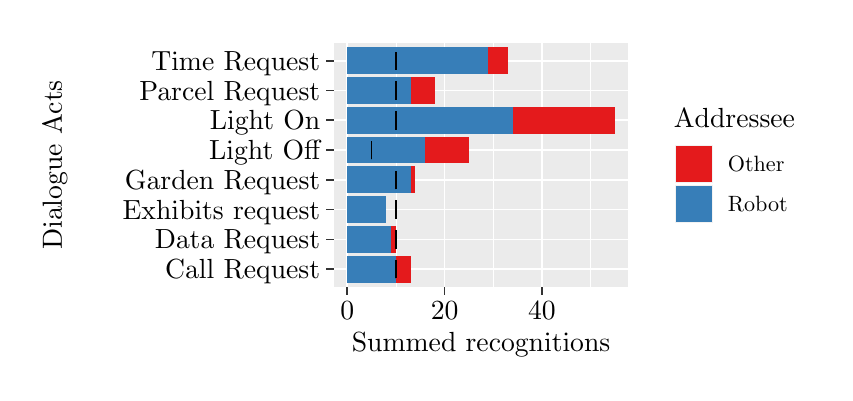
\begin{tikzpicture}[x=1pt,y=1pt]
\definecolor{fillColor}{RGB}{255,255,255}
\path[use as bounding box,fill=fillColor,fill opacity=0.00] (0,0) rectangle (288.00,124.59);
\begin{scope}
\path[clip] (  0.00,  0.00) rectangle (288.00,124.59);
\definecolor{drawColor}{RGB}{255,255,255}
\definecolor{fillColor}{RGB}{255,255,255}

\path[draw=drawColor,line width= 0.6pt,line join=round,line cap=round,fill=fillColor] (  0.00,  0.00) rectangle (288.00,124.59);
\end{scope}
\begin{scope}
\path[clip] (110.65, 30.86) rectangle (217.04,119.09);
\definecolor{fillColor}{gray}{0.92}

\path[fill=fillColor] (110.65, 30.86) rectangle (217.04,119.09);
\definecolor{drawColor}{RGB}{255,255,255}

\path[draw=drawColor,line width= 0.3pt,line join=round] (133.07, 30.86) --
	(133.07,119.09);

\path[draw=drawColor,line width= 0.3pt,line join=round] (168.24, 30.86) --
	(168.24,119.09);

\path[draw=drawColor,line width= 0.3pt,line join=round] (203.41, 30.86) --
	(203.41,119.09);

\path[draw=drawColor,line width= 0.6pt,line join=round] (110.65, 37.32) --
	(217.04, 37.32);

\path[draw=drawColor,line width= 0.6pt,line join=round] (110.65, 48.08) --
	(217.04, 48.08);

\path[draw=drawColor,line width= 0.6pt,line join=round] (110.65, 58.84) --
	(217.04, 58.84);

\path[draw=drawColor,line width= 0.6pt,line join=round] (110.65, 69.60) --
	(217.04, 69.60);

\path[draw=drawColor,line width= 0.6pt,line join=round] (110.65, 80.36) --
	(217.04, 80.36);

\path[draw=drawColor,line width= 0.6pt,line join=round] (110.65, 91.11) --
	(217.04, 91.11);

\path[draw=drawColor,line width= 0.6pt,line join=round] (110.65,101.87) --
	(217.04,101.87);

\path[draw=drawColor,line width= 0.6pt,line join=round] (110.65,112.63) --
	(217.04,112.63);

\path[draw=drawColor,line width= 0.6pt,line join=round] (115.49, 30.86) --
	(115.49,119.09);

\path[draw=drawColor,line width= 0.6pt,line join=round] (150.66, 30.86) --
	(150.66,119.09);

\path[draw=drawColor,line width= 0.6pt,line join=round] (185.83, 30.86) --
	(185.83,119.09);
\definecolor{fillColor}{RGB}{55,126,184}

\path[fill=fillColor] (115.49, 32.48) rectangle (133.07, 42.16);
\definecolor{fillColor}{RGB}{228,26,28}

\path[fill=fillColor] (133.07, 32.48) rectangle (138.35, 42.16);
\definecolor{fillColor}{RGB}{55,126,184}

\path[fill=fillColor] (115.49, 43.24) rectangle (131.31, 52.92);
\definecolor{fillColor}{RGB}{228,26,28}

\path[fill=fillColor] (131.31, 43.24) rectangle (133.07, 52.92);
\definecolor{fillColor}{RGB}{55,126,184}

\path[fill=fillColor] (115.49, 53.99) rectangle (129.56, 63.68);

\path[fill=fillColor] (115.49, 64.75) rectangle (138.35, 74.44);
\definecolor{fillColor}{RGB}{228,26,28}

\path[fill=fillColor] (138.35, 64.75) rectangle (140.11, 74.44);
\definecolor{fillColor}{RGB}{55,126,184}

\path[fill=fillColor] (115.49, 75.51) rectangle (143.62, 85.20);
\definecolor{fillColor}{RGB}{228,26,28}

\path[fill=fillColor] (143.62, 75.51) rectangle (159.45, 85.20);
\definecolor{fillColor}{RGB}{55,126,184}

\path[fill=fillColor] (115.49, 86.27) rectangle (175.28, 95.96);
\definecolor{fillColor}{RGB}{228,26,28}

\path[fill=fillColor] (175.28, 86.27) rectangle (212.20, 95.96);
\definecolor{fillColor}{RGB}{55,126,184}

\path[fill=fillColor] (115.49, 97.03) rectangle (138.35,106.72);
\definecolor{fillColor}{RGB}{228,26,28}

\path[fill=fillColor] (138.35, 97.03) rectangle (147.14,106.72);
\definecolor{fillColor}{RGB}{55,126,184}

\path[fill=fillColor] (115.49,107.79) rectangle (166.48,117.47);
\definecolor{fillColor}{RGB}{228,26,28}

\path[fill=fillColor] (166.48,107.79) rectangle (173.52,117.47);
\definecolor{drawColor}{RGB}{0,0,0}

\path[draw=drawColor,line width= 0.6pt,line join=round] (133.07, 33.99) --
	(133.07, 40.64);

\path[draw=drawColor,line width= 0.6pt,line join=round] (133.07, 37.32) --
	(133.07, 37.32);

\path[draw=drawColor,line width= 0.6pt,line join=round] (133.07, 33.99) --
	(133.07, 40.64);

\path[draw=drawColor,line width= 0.6pt,line join=round] (133.07, 33.99) --
	(133.07, 40.64);

\path[draw=drawColor,line width= 0.6pt,line join=round] (133.07, 37.32) --
	(133.07, 37.32);

\path[draw=drawColor,line width= 0.6pt,line join=round] (133.07, 33.99) --
	(133.07, 40.64);

\path[draw=drawColor,line width= 0.6pt,line join=round] (133.07, 44.75) --
	(133.07, 51.40);

\path[draw=drawColor,line width= 0.6pt,line join=round] (133.07, 48.08) --
	(133.07, 48.08);

\path[draw=drawColor,line width= 0.6pt,line join=round] (133.07, 44.75) --
	(133.07, 51.40);

\path[draw=drawColor,line width= 0.6pt,line join=round] (133.07, 44.75) --
	(133.07, 51.40);

\path[draw=drawColor,line width= 0.6pt,line join=round] (133.07, 48.08) --
	(133.07, 48.08);

\path[draw=drawColor,line width= 0.6pt,line join=round] (133.07, 44.75) --
	(133.07, 51.40);

\path[draw=drawColor,line width= 0.6pt,line join=round] (133.07, 55.51) --
	(133.07, 62.16);

\path[draw=drawColor,line width= 0.6pt,line join=round] (133.07, 58.84) --
	(133.07, 58.84);

\path[draw=drawColor,line width= 0.6pt,line join=round] (133.07, 55.51) --
	(133.07, 62.16);

\path[draw=drawColor,line width= 0.6pt,line join=round] (133.07, 66.27) --
	(133.07, 72.92);

\path[draw=drawColor,line width= 0.6pt,line join=round] (133.07, 69.60) --
	(133.07, 69.60);

\path[draw=drawColor,line width= 0.6pt,line join=round] (133.07, 66.27) --
	(133.07, 72.92);

\path[draw=drawColor,line width= 0.6pt,line join=round] (133.07, 66.27) --
	(133.07, 72.92);

\path[draw=drawColor,line width= 0.6pt,line join=round] (133.07, 69.60) --
	(133.07, 69.60);

\path[draw=drawColor,line width= 0.6pt,line join=round] (133.07, 66.27) --
	(133.07, 72.92);

\path[draw=drawColor,line width= 0.6pt,line join=round] (124.28, 77.03) --
	(124.28, 83.68);

\path[draw=drawColor,line width= 0.6pt,line join=round] (124.28, 80.36) --
	(124.28, 80.36);

\path[draw=drawColor,line width= 0.6pt,line join=round] (124.28, 77.03) --
	(124.28, 83.68);

\path[draw=drawColor,line width= 0.6pt,line join=round] (124.28, 77.03) --
	(124.28, 83.68);

\path[draw=drawColor,line width= 0.6pt,line join=round] (124.28, 80.36) --
	(124.28, 80.36);

\path[draw=drawColor,line width= 0.6pt,line join=round] (124.28, 77.03) --
	(124.28, 83.68);

\path[draw=drawColor,line width= 0.6pt,line join=round] (133.07, 87.79) --
	(133.07, 94.44);

\path[draw=drawColor,line width= 0.6pt,line join=round] (133.07, 91.11) --
	(133.07, 91.11);

\path[draw=drawColor,line width= 0.6pt,line join=round] (133.07, 87.79) --
	(133.07, 94.44);

\path[draw=drawColor,line width= 0.6pt,line join=round] (133.07, 87.79) --
	(133.07, 94.44);

\path[draw=drawColor,line width= 0.6pt,line join=round] (133.07, 91.11) --
	(133.07, 91.11);

\path[draw=drawColor,line width= 0.6pt,line join=round] (133.07, 87.79) --
	(133.07, 94.44);

\path[draw=drawColor,line width= 0.6pt,line join=round] (133.07, 98.55) --
	(133.07,105.20);

\path[draw=drawColor,line width= 0.6pt,line join=round] (133.07,101.87) --
	(133.07,101.87);

\path[draw=drawColor,line width= 0.6pt,line join=round] (133.07, 98.55) --
	(133.07,105.20);

\path[draw=drawColor,line width= 0.6pt,line join=round] (133.07, 98.55) --
	(133.07,105.20);

\path[draw=drawColor,line width= 0.6pt,line join=round] (133.07,101.87) --
	(133.07,101.87);

\path[draw=drawColor,line width= 0.6pt,line join=round] (133.07, 98.55) --
	(133.07,105.20);

\path[draw=drawColor,line width= 0.6pt,line join=round] (133.07,109.31) --
	(133.07,115.96);

\path[draw=drawColor,line width= 0.6pt,line join=round] (133.07,112.63) --
	(133.07,112.63);

\path[draw=drawColor,line width= 0.6pt,line join=round] (133.07,109.31) --
	(133.07,115.96);

\path[draw=drawColor,line width= 0.6pt,line join=round] (133.07,109.31) --
	(133.07,115.96);

\path[draw=drawColor,line width= 0.6pt,line join=round] (133.07,112.63) --
	(133.07,112.63);

\path[draw=drawColor,line width= 0.6pt,line join=round] (133.07,109.31) --
	(133.07,115.96);
\end{scope}
\begin{scope}
\path[clip] (  0.00,  0.00) rectangle (288.00,124.59);
\definecolor{drawColor}{RGB}{0,0,0}

\node[text=drawColor,anchor=base east,inner sep=0pt, outer sep=0pt, scale=  1.00] at (105.70, 33.87) {Call Request};

\node[text=drawColor,anchor=base east,inner sep=0pt, outer sep=0pt, scale=  1.00] at (105.70, 44.63) {Data Request};

\node[text=drawColor,anchor=base east,inner sep=0pt, outer sep=0pt, scale=  1.00] at (105.70, 55.39) {Exhibits request};

\node[text=drawColor,anchor=base east,inner sep=0pt, outer sep=0pt, scale=  1.00] at (105.70, 66.15) {Garden Request};

\node[text=drawColor,anchor=base east,inner sep=0pt, outer sep=0pt, scale=  1.00] at (105.70, 76.91) {Light Off};

\node[text=drawColor,anchor=base east,inner sep=0pt, outer sep=0pt, scale=  1.00] at (105.70, 87.67) {Light On};

\node[text=drawColor,anchor=base east,inner sep=0pt, outer sep=0pt, scale=  1.00] at (105.70, 98.43) {Parcel Request};

\node[text=drawColor,anchor=base east,inner sep=0pt, outer sep=0pt, scale=  1.00] at (105.70,109.19) {Time Request};
\end{scope}
\begin{scope}
\path[clip] (  0.00,  0.00) rectangle (288.00,124.59);
\definecolor{drawColor}{gray}{0.20}

\path[draw=drawColor,line width= 0.6pt,line join=round] (107.90, 37.32) --
	(110.65, 37.32);

\path[draw=drawColor,line width= 0.6pt,line join=round] (107.90, 48.08) --
	(110.65, 48.08);

\path[draw=drawColor,line width= 0.6pt,line join=round] (107.90, 58.84) --
	(110.65, 58.84);

\path[draw=drawColor,line width= 0.6pt,line join=round] (107.90, 69.60) --
	(110.65, 69.60);

\path[draw=drawColor,line width= 0.6pt,line join=round] (107.90, 80.36) --
	(110.65, 80.36);

\path[draw=drawColor,line width= 0.6pt,line join=round] (107.90, 91.11) --
	(110.65, 91.11);

\path[draw=drawColor,line width= 0.6pt,line join=round] (107.90,101.87) --
	(110.65,101.87);

\path[draw=drawColor,line width= 0.6pt,line join=round] (107.90,112.63) --
	(110.65,112.63);
\end{scope}
\begin{scope}
\path[clip] (  0.00,  0.00) rectangle (288.00,124.59);
\definecolor{drawColor}{gray}{0.20}

\path[draw=drawColor,line width= 0.6pt,line join=round] (115.49, 28.11) --
	(115.49, 30.86);

\path[draw=drawColor,line width= 0.6pt,line join=round] (150.66, 28.11) --
	(150.66, 30.86);

\path[draw=drawColor,line width= 0.6pt,line join=round] (185.83, 28.11) --
	(185.83, 30.86);
\end{scope}
\begin{scope}
\path[clip] (  0.00,  0.00) rectangle (288.00,124.59);
\definecolor{drawColor}{RGB}{0,0,0}

\node[text=drawColor,anchor=base,inner sep=0pt, outer sep=0pt, scale=  1.00] at (115.49, 19.03) {0};

\node[text=drawColor,anchor=base,inner sep=0pt, outer sep=0pt, scale=  1.00] at (150.66, 19.03) {20};

\node[text=drawColor,anchor=base,inner sep=0pt, outer sep=0pt, scale=  1.00] at (185.83, 19.03) {40};
\end{scope}
\begin{scope}
\path[clip] (  0.00,  0.00) rectangle (288.00,124.59);
\definecolor{drawColor}{RGB}{0,0,0}

\node[text=drawColor,anchor=base,inner sep=0pt, outer sep=0pt, scale=  1.00] at (163.85,  7.44) {Summed recognitions};
\end{scope}
\begin{scope}
\path[clip] (  0.00,  0.00) rectangle (288.00,124.59);
\definecolor{drawColor}{RGB}{0,0,0}

\node[text=drawColor,rotate= 90.00,anchor=base,inner sep=0pt, outer sep=0pt, scale=  1.00] at ( 12.39, 74.98) {Dialogue Acts};
\end{scope}
\begin{scope}
\path[clip] (  0.00,  0.00) rectangle (288.00,124.59);
\definecolor{fillColor}{RGB}{255,255,255}

\path[fill=fillColor] (228.04, 48.11) rectangle (282.50,101.85);
\end{scope}
\begin{scope}
\path[clip] (  0.00,  0.00) rectangle (288.00,124.59);
\definecolor{drawColor}{RGB}{0,0,0}

\node[text=drawColor,anchor=base west,inner sep=0pt, outer sep=0pt, scale=  1.00] at (233.54, 88.49) {Addressee};
\end{scope}
\begin{scope}
\path[clip] (  0.00,  0.00) rectangle (288.00,124.59);
\definecolor{drawColor}{RGB}{255,255,255}
\definecolor{fillColor}{gray}{0.95}

\path[draw=drawColor,line width= 0.6pt,line join=round,line cap=round,fill=fillColor] (233.54, 68.06) rectangle (247.99, 82.51);
\end{scope}
\begin{scope}
\path[clip] (  0.00,  0.00) rectangle (288.00,124.59);
\definecolor{fillColor}{RGB}{228,26,28}

\path[fill=fillColor] (234.25, 68.77) rectangle (247.28, 81.80);
\end{scope}
\begin{scope}
\path[clip] (  0.00,  0.00) rectangle (288.00,124.59);
\definecolor{drawColor}{RGB}{255,255,255}
\definecolor{fillColor}{gray}{0.95}

\path[draw=drawColor,line width= 0.6pt,line join=round,line cap=round,fill=fillColor] (233.54, 53.61) rectangle (247.99, 68.06);
\end{scope}
\begin{scope}
\path[clip] (  0.00,  0.00) rectangle (288.00,124.59);
\definecolor{fillColor}{RGB}{55,126,184}

\path[fill=fillColor] (234.25, 54.32) rectangle (247.28, 67.35);
\end{scope}
\begin{scope}
\path[clip] (  0.00,  0.00) rectangle (288.00,124.59);
\definecolor{drawColor}{RGB}{0,0,0}

\node[text=drawColor,anchor=base west,inner sep=0pt, outer sep=0pt, scale=  0.80] at (252.99, 72.53) {Other};
\end{scope}
\begin{scope}
\path[clip] (  0.00,  0.00) rectangle (288.00,124.59);
\definecolor{drawColor}{RGB}{0,0,0}

\node[text=drawColor,anchor=base west,inner sep=0pt, outer sep=0pt, scale=  0.80] at (252.99, 58.08) {Robot};
\end{scope}
\end{tikzpicture}
